\originalchapter{作业十一：低能谱、载流子与氦}
\psource{8.044，2013 春，PS11，5 月 10 日截止。中文题面；据官方答案核对的 AI 独立解答。}
\originalsection{1．表面波量子 ripplon}
\begin{exercise}
液体--蒸气界面的二维波各只有法向一个偏振，能量 $\epsilon=\hbar\omega=bk^{3/2}$。矩形面 $L_x,L_y$ 取周期边界，$\vct k=(2\pi m/L_x,2\pi n/L_y)$，$m,n\in\mathbb Z$。
(a) 求每 $\dd k_x\dd k_y$ 的波矢密度；(b) 求能量态密度并画图；(c) 恒面积热容留成无量纲积分，指出温度幂次并画图；(d) 是否有能隙行为？
\end{exercise}
\begin{solution}
(a) $D_k=A/(2\pi)^2$。(b) $\mathcal N(\epsilon)=A(\epsilon/b)^{4/3}/(4\pi)$，$D(\epsilon)=A\epsilon^{1/3}/(3\pi b^{4/3})$，从原点按三分之一次幂上升。
(c) 零点能有高频截止且恒面积不贡献热容。激发部分
\[C_A=\frac{A\kb(\kb T)^{4/3}}{3\pi b^{4/3}}\int_0^\infty\frac{x^{7/3}e^x}{(e^x-1)^2}\dd x\propto T^{4/3}.\]
分部积分亦得 $7/3$ 倍 $\int x^{4/3}/(e^x-1)\dd x$；官方第一条热容积分误保留零点 $1/2$，此项求温度导数必须消失。(d) 无限界面低波数能量趋零，无能隙；有限尺寸最低非零波数提供极低温截止。连续谱近似须处于此有限尺寸尺度以上、模型高频截止以下。
\end{solution}
\begin{center}\begin{tikzpicture}\begin{axis}[width=6.5cm,height=3.5cm,xmin=0,xmax=3,ymin=0,ymax=1.6,xlabel={无量纲能量},ylabel={归一化 $D$}]\addplot[domain=0:3,thick]{x^(1/3)};\end{axis}\end{tikzpicture}\hspace{.3cm}\begin{tikzpicture}\begin{axis}[width=6.5cm,height=3.5cm,xmin=0,xmax=2,ymin=0,ymax=2.7,xlabel={无量纲温度},ylabel={归一化 $C_A$}]\addplot[domain=0:2,thick]{x^(4/3)};\end{axis}\end{tikzpicture}\end{center}
\originalsection{2．方锥色散的二维金属}
\begin{exercise}
方形样品边长 $L$，周期势中的电子态仍以波矢标记。原图等能线为边\textbf{平行} $k_x,k_y$ 的正方形，能量沿正 $k_x$ 为 $\gamma k_x$；等价 $\epsilon=\gamma\max(|k_x|,|k_y|)$，$\gamma>0$。
(a) 周期边界允许波矢；(b) 波矢密度；(c) 含电子自旋的 $D(\epsilon)$，画图；(d) $N$ 电子的零温 Fermi 能；(e) 零温总能；(f) 无计算判断低温热容幂次；(g) 零温表面张力（铺展压的负值）。
\end{exercise}
\begin{solution}
(a) $\vct k=(2\pi/L)(m,n)$，$m,n\in\mathbb Z$，含零值。(b) $D_k=A/(2\pi)^2$。(c) 等能内面积 $4(\epsilon/\gamma)^2$，自旋二重，$\mathcal N=2A\epsilon^2/(\pi^2\gamma^2)$，$D=4A\epsilon/(\pi^2\gamma^2)$：从原点线性增长。
(d) $\epsilon_F=\pi\gamma\sqrt{N/(2A)}$。(e) $U=2N\epsilon_F/3$。(f) Fermi 面附近被热激发的比例 $\sim T$、每粒增能 $\sim T$，故 $C\sim T$。(g) 固定 $N$，$\epsilon_F\propto A^{-1/2}$，$\mathcal S=U_A=-N\epsilon_F/(3A)$。若把原图误当对角线菱形，态密度会错一倍。
\end{solution}
\begin{center}\begin{tikzpicture}[scale=.9]\draw[->](-1.8,0)--(1.9,0)node[right]{$k_x$};\draw[->](0,-1.7)--(0,1.8)node[above]{$k_y$};\draw[thick](-1,-1)rectangle(1,1);\node[above]at(1,1){$\epsilon/\gamma$};\end{tikzpicture}\hspace{1cm}\begin{tikzpicture}\begin{axis}[width=6cm,height=3.5cm,xmin=0,xmax=2,ymin=0,ymax=2,xlabel={能量},ylabel={$D$/斜率}]\addplot[domain=0:2,thick]{x};\end{axis}\end{tikzpicture}\end{center}
\originalsection{3．半导体施主态}
\begin{exercise}
忽略价带，$N_D$ 个施主能级置于零，每态至多一电子；导带底 $\Delta>0$，初态施主全满、导带空，DOS
\[D(\epsilon)=N_D\delta(\epsilon)+\frac V{2\pi^2}\left(\frac{2m_e}{\hbar^2}\right)^{3/2}\sqrt{\epsilon-\Delta}\,\Theta(\epsilon-\Delta).\]
假定 $\Delta\gg\kb T$ 且导带为非简并。
(a) 定义 $\alpha(T)$ 使 $N_C=\alpha e^{-\Delta/(\kb T)}e^{\mu/(\kb T)}$，证明 $\alpha\propto T^{3/2}$；(b) 给施主恰半空的温度方程，不要求解；(c) 极低温在 $0,\Delta$ 中间近似求 $\mu(T)$，用 $T\ln T\to0$ 得其零温极限；(d) 保留施主 Fermi 函数，消去 $e^{-\beta\mu}$，证明 $y^2+qy-q=0$，$y=N_C/N_D,q=\alpha e^{-\beta\Delta}/N_D$，检验半空点及低/高温趋势。
\end{exercise}
\begin{solution}
(a) 导带 Boltzmann 积分给 $\alpha=2V/\lambda_T^3=V(2m_e\kb T/\hbar^2)^{3/2}/(4\pi^{3/2})$。
(b) 施主半满时 $\mu=0$、$N_C=N_D/2$，故 $\alpha(T)e^{-\Delta/(\kb T)}=N_D/2$。
(c) 空施主数 $N_De^{-\beta\mu}$，与导带数相等，$\mu=\Delta/2+(\kb T/2)\ln[N_D/\alpha(T)]\to\Delta/2$。严格 $T=0$ 任意隙内化学势都给相同占据，这里选的是固定总数有限温极限。
(d) 施主数 $N_D/(1+e^{-\beta\mu})$，用 $e^{-\beta\mu}=\alpha e^{-\beta\Delta}/N_C=q/y$ 和数守恒得所求式。$y=1/2$ 要求 $q=1/2$，与 (b) 同；$q\to0$ 给 $y\to0$，$q\to\infty$ 时由 $y^2/q+y-1=0$ 给 $y\to1$。后者是简化方程的形式高温趋势，已超出开头 $\Delta\gg\kb T$ 及忽略价带的条件，不构成真实半导体全温证明。原卷“施主先升至价带”为文字笔误，应为导带。
\end{solution}
\originalsection{4．完全自旋极化}
\begin{exercise}
三维理想自旋 $1/2$ 费米气体，$\epsilon=\hbar^2k^2/(2m)-2\mu_0Hm_s$，$m_s=\pm1/2$。
(a) 各自旋 DOS 并画总 DOS；(b) 零温全部粒子进入低能自旋的最低场强；(c) 铜电子 $\mu_0=-9.27\times10^{-21}$ erg/G、$m=9.11\times10^{-28}$ g、$n=8.45\times10^{22}$ cm$^{-3}$，算 Tesla；(d) 液 $^3$He 核 $\mu_0=1.075\times10^{-23}$ erg/G、$m=5.01\times10^{-24}$ g、$n=1.64\times10^{22}$ cm$^{-3}$，同算。原卷列实验磁场仅作当时可达量级比较。
\end{exercise}
\begin{solution}
(a) 设 $C=V(2m/\hbar^2)^{3/2}/(4\pi^2)$，$D_+=C\sqrt{\epsilon+\mu_0H}\Theta(\epsilon+\mu_0H)$、$D_-=C\sqrt{\epsilon-\mu_0H}\Theta(\epsilon-\mu_0H)$；总 DOS 在两阈值 $\pm|\mu_0H|$ 开始两支，第二支起点有平方根尖斜率。
(b) 极化后单自旋 Fermi 动能为 $\hbar^2(6\pi^2n)^{2/3}/(2m)$，要不碰到另一支，需 $2|\mu_0|H$ 至少为此值，
\[H_0=\frac{\hbar^2(6\pi^2n)^{2/3}}{4m|\mu_0|}.\]
负磁矩改变哪支低，不使场强为负。(c)(d) 用 $\hbar=1.054571817\times10^{-27}$ erg s 实算约 $9.63\times10^4$ T、$5.06\times10^3$ T；是理想模型尺度，液氦相互作用及电子能带会改变真实响应。
\end{solution}
\begin{center}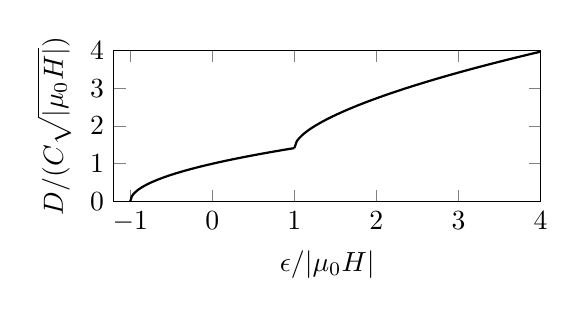
\begin{tikzpicture}\begin{axis}[width=7cm,height=3.5cm,xmin=-1.2,xmax=4,ymin=0,ymax=4,xlabel={$\epsilon/|\mu_0H|$},ylabel={$D/(C\sqrt{|\mu_0H|})$},samples=100]\addplot[domain=-1:1,thick]{sqrt(x+1)};\addplot[domain=1:4,thick]{sqrt(x+1)+sqrt(x-1)};\end{axis}\end{tikzpicture}\end{center}
\originalsection{5．零温氦同位素溶解度}
\begin{exercise}
低温混合物分为富 $^4$He 与富 $^3$He 相；零温后一相为纯 $^3$He，前一相仍能溶一定浓度。简化图中，向富 $^4$He 加一个 $^3$He 的势能比加入纯 $^3$He 低 $W>0$；溶入的自旋 $1/2$ 原子作有效质量 $m^*$ 的理想费米粒子，动能 $\hbar^2k^2/(2m^*)$。
(a) 求最大 $n_3$；(b) 用题给 $\hbar\simeq10^{-27}$ erg s、$\kb\simeq10^{-16}$ erg/K、$m^*\simeq10\times10^{-24}$ g、$W/\kb\simeq.5$ K、$n_4\simeq2\times10^{22}$ cm$^{-3}$ 算 $x_c=n_3/(n_3+n_4)$。
\end{exercise}
\begin{solution}
加粒子代价为势底加化学势，满溶时 $\epsilon_F=W$。故 $n_{3,\max}=(2m^*W/\hbar^2)^{3/2}/(3\pi^2)$；不是令平均动能等于 $W$。代题设粗常数得 $n_{3,\max}\simeq1.068\times10^{21}$ cm$^{-3}$、$x_c\simeq5.07\%$，与原图量级相符。本模型将纯相加粒子基准设为零，$W$ 是有效化学势差，不是可直接从裸 pair 势推出的测量。
\end{solution}
\originalsection{6．$^3$He 熔化线}
\begin{exercise}
熔化图分低温 I、中温 II、高温 III。II 中液体近似零温自旋 $1/2$ 费米气体，固体近似固定各晶格位、无场非相互作用自旋；I 中固体反铁磁有序，等效局域场满足 $\mu H_{\rm eff}\gg\kb T$。
(a) II 中液体熵；(b) II 中固体熵；(c) I 中近零温固体熵；(d)(e) 用 $\dd P_M/\dd T=(S_l-S_s)/(N\Delta v_0)$，$\Delta v_0>0$ 常数，求 II、I 斜率；(f) 在 II 两相共存线上加热，熔化还是凝固，为什么？
\end{exercise}
\begin{solution}
(a) 题设零温近似 $S_l=0$；实际小温度有线性修正。(b) 每位两自旋态，$S_s=N\kb\ln2$。(c) 有序基本非简并，$S_s\to0$；有限整体有序方向简并不产生广延熵。(d) II 斜率 $-\kb\ln2/\Delta v_0<0$。(e) I 的零温极限两熵皆零，斜率趋零；题设不足以确定全部有限温曲线。(f) 固体单位粒子熵较大，吸热增加熵可将液体转为固体，故凝固，潜热 $T(S_s-S_l)>0$。这是共存线上转换，不能忽略约束而声称任意加热都凝固。
\end{solution}
